% Standalone source for figures/fig-rhetoric-shapes.pdf
% Build: pdflatex fig-rhetoric-shapes.tex  (run inside figures/)
\documentclass[tikz,border=6pt]{standalone}
\usepackage{tikz}
\usetikzlibrary{arrows.meta,positioning,calc}
\begin{document}
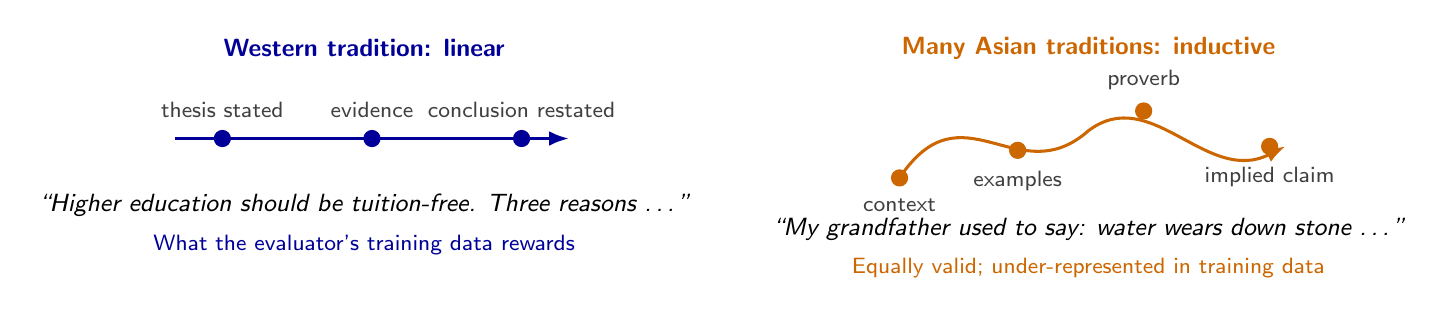
\begin{tikzpicture}[
  font=\sffamily\small,
  node/.style={circle,fill=#1,inner sep=2.2pt},
  lbl/.style={font=\sffamily\footnotesize,text=black!75},
  quote/.style={font=\sffamily\small\itshape}
]
% ---------- Left: Anglo-American linear pattern
\node[font=\sffamily\bfseries\small,text=blue!60!black] at (0,2.35) {Western tradition: linear};
\draw[-{Latex[length=2.5mm]},line width=1.1pt,blue!60!black] (-2.4,1.2) -- (2.6,1.2);
\foreach \x/\t in {-1.8/thesis stated, 0.1/evidence, 2.0/conclusion restated}{
  \node[node=blue!60!black] at (\x,1.2) {};
  \node[lbl,above=4pt] at (\x,1.2) {\t};
}
\node[quote] at (0,0.35) {``Higher education should be tuition-free. Three reasons \ldots''};
\node[lbl,text=blue!60!black] at (0,-0.15) {What the evaluator's training data rewards};

% ---------- Right: inductive / context-first pattern
\begin{scope}[xshift=9.2cm]
\node[font=\sffamily\bfseries\small,text=orange!80!black] at (0,2.35) {Many Asian traditions: inductive};
\draw[-{Latex[length=2.5mm]},line width=1.1pt,orange!80!black]
  (-2.4,0.7) .. controls (-1.6,1.9) and (-0.9,0.5) .. (0.0,1.3)
             .. controls (0.8,1.9) and (1.5,0.6) .. (2.5,1.1);
\foreach \x/\y/\t/\p in {-2.4/0.7/context/below, -0.9/1.05/examples/below, 0.7/1.55/proverb/above, 2.3/1.1/implied claim/below}{
  \node[node=orange!80!black] at (\x,\y) {};
  \node[lbl,\p=4pt] at (\x,\y) {\t};
}
\node[quote] at (0,0.05) {``My grandfather used to say: water wears down stone \ldots''};
\node[lbl,text=orange!80!black] at (0,-0.45) {Equally valid; under-represented in training data};
\end{scope}
\end{tikzpicture}
\end{document}
